As for the use of light microscopes, there are several techniques and configurations which are achieved by varying the amount of lenses and light sources: bright-field, dark-field, phase-contrast, differential interference and fluorescence \cite{roane2009microscopic}. As stated by \citeonline{lawlor2019introduction}, images in bright-field microscopy are characterized by the contrast between the sample and the bright white background, generated by transmitted light. It is commonly used in pathology and histology fields for imaging fixed cells and tissues to reveal their structure, shape, and organization. The amount of light should be controlled, since the sample might suffer substantial changes, e.g. the chlorophyll molecules when illuminated by UV and visible light suffer irreversible breakdown (photodegradation) and generate other photoproducts \cite{petrovic2017clorophyll}. The \autoref{fig:bright-field_microscopy} provides an example of bright-field microscopy image.

\begin{figure}[htb]
	\centering
	\caption{\label{fig:bright-field_microscopy} Example of bright-field microscopy image of bone tissue.}
	\begin{center}
	    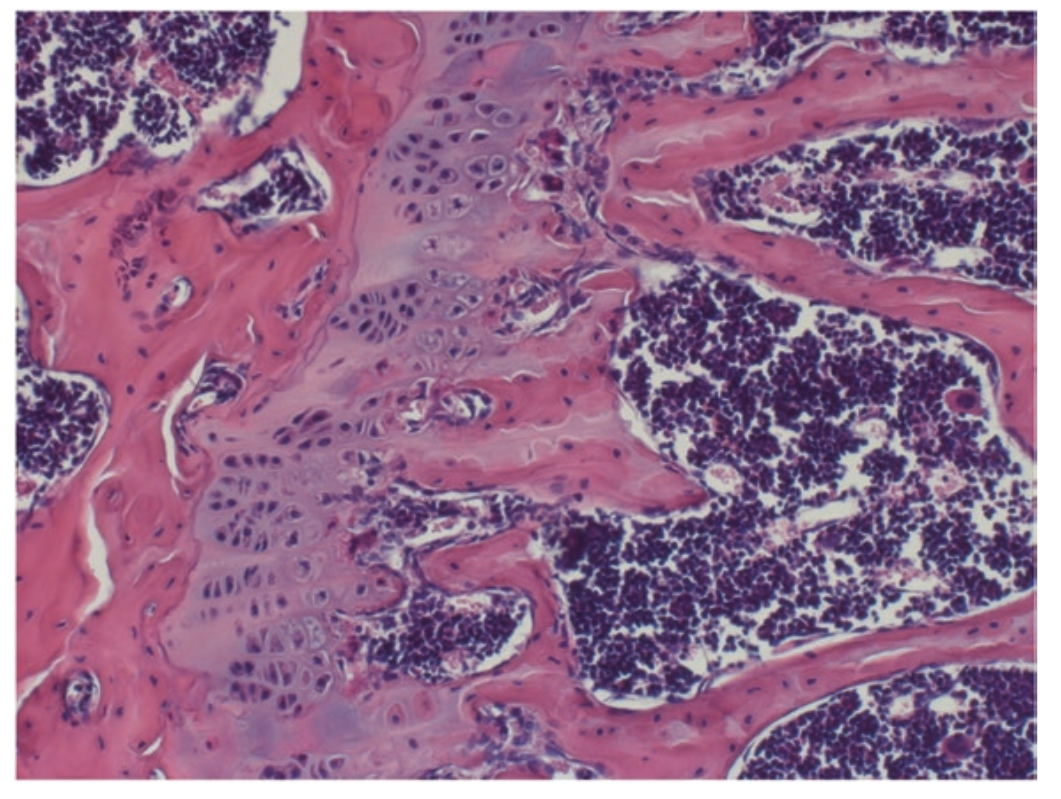
\includegraphics[scale=0.25]{images/bright-field_microscopy.png}
	\end{center}
	\centering
    \fdireta{lawlor2019introduction}
\end{figure}

\subsection{Z-stacking technique}

The \textit{z-stacking} is a procedure to capture images in different positions concerning the $z$ axis, named slices, which may create a pseudo 3D image of the sample and consequently retrieve depth information about the specimen \cite{lawlor2019introduction}. \autoref{fig:z-stack-scheme} presents the scheme of a z-stack acquisition with an arbitrary object:

\begin{figure}[htb]
	\centering
	\caption{\label{fig:z-stack-scheme} Scheme of a z-stack image dataset acquisition with an arbritrary object.}
	\begin{center}
	    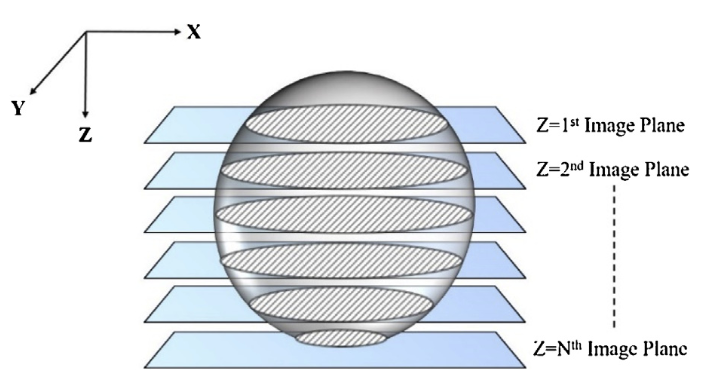
\includegraphics[scale=0.4]{images/z-stack-object.png}
	\end{center}
	\centering
    \fdireta{trivedi2020centroid}
\end{figure}

The distance between each slice is dictated manually or automatically by the technique, and the focus needs to be adjusted at each slice. Next, the images must be aligned before any analysis is conducted. \autoref{fig:z-stack_example} represents the differences in focus between the slices of a z-stack.

\begin{figure}[htb]
	\centering
	\caption{\label{fig:z-stack_example} Z-stack images of yeast cells, acquired in positions under the focal plane (-15, -10 and -5 $\mu m$), exactly on it (0 $\mu m$) and above it (5, 10 and 15 $\mu m$).}
	\begin{center}
	    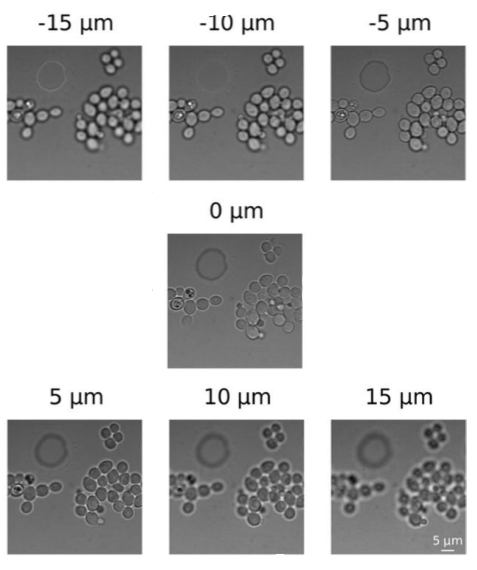
\includegraphics[scale=0.5]{images/z-stack.png}
	\end{center}
	\centering
    \fdireta{wei2018neural}
\end{figure}